\documentclass[11pt,a4paper]{ctexart}
\usepackage[a4paper,margin=1.75cm,headheight=15pt]{geometry}
\usepackage{amsmath,amssymb,mathtools,booktabs,tabularx,array,enumitem}
\usepackage[most]{tcolorbox}
\usepackage{tikz}
\usetikzlibrary{arrows.meta,positioning,calc,fit}
\usepackage{xcolor,fancyhdr,hyperref,microtype,lastpage}
\newcolumntype{Y}{>{\raggedright\arraybackslash}X}
\newcolumntype{L}[1]{>{\raggedright\arraybackslash}p{#1}}
\newcolumntype{C}[1]{>{\centering\arraybackslash}p{#1}}
\setlength{\parindent}{2em}
\setlength{\parskip}{0.34em}
\setlength{\emergencystretch}{3em}
\renewcommand{\arraystretch}{1.2}
\setlength{\tabcolsep}{3pt}
\setlist[itemize]{itemsep=0.18em,topsep=0.35em,leftmargin=2em}
\setlist[enumerate]{itemsep=0.18em,topsep=0.35em,leftmargin=2em}
\definecolor{deep}{RGB}{35,64,76}
\definecolor{soft}{RGB}{244,247,247}
\definecolor{greenish}{RGB}{49,91,73}
\definecolor{warnc}{RGB}{137,61,55}
\definecolor{purple}{RGB}{82,72,112}
\definecolor{rulegray}{RGB}{108,114,118}
\hypersetup{colorlinks=true,linkcolor=deep,urlcolor=purple,pdftitle={NET-04 IP 地址、子网与分组转发}}
\pagestyle{fancy}
\fancyhf{}
\lhead{\small\color{deep}\textbf{408 · 计算机网络 NET-04}}
\rhead{\small\color{deep}Scope · Prefix · Next Hop · Rewrite}
\cfoot{\small 第 \thepage\ 页 / 共 \pageref{LastPage} 页}
\renewcommand{\headrulewidth}{0.4pt}
\newtcolorbox{corebox}[1]{breakable,colback=soft,colframe=deep,title=\textbf{#1},boxrule=0.8pt,arc=2mm}
\newtcolorbox{methodbox}[1]{breakable,colback=white,colframe=greenish,title=\textbf{#1},boxrule=0.7pt,arc=1.5mm}
\newtcolorbox{warnbox}[1]{breakable,colback=white,colframe=warnc,title=\textbf{#1},boxrule=0.7pt,arc=1.5mm}
\newtcolorbox{examplebox}[1]{breakable,colback=white,colframe=purple,title=\textbf{#1},boxrule=0.7pt,arc=1.5mm}
\newcommand{\kw}[1]{\textbf{\color{deep}#1}}
\newcommand{\code}[1]{\texttt{#1}}
\tikzset{net/.style={draw=deep,rounded corners=1.5mm,text width=2.7cm,minimum height=0.95cm,align=center,fill=soft,font=\small,inner sep=3pt},flow/.style={-{Latex[length=2mm]},thick,draw=deep},ref/.style={-{Latex[length=2mm]},dashed,draw=rulegray}}

\title{\vspace{-1.1cm}\textbf{IP 地址、子网与分组转发}\\[0.4em]\large 怎样把全局目的压缩成每一跳的局部动作}
\author{408 · 计算机网络 Topic NET-04}
\date{}

\begin{document}
\maketitle

\begin{corebox}{母问题：路由器不知道整条旅程，为什么仍能把分组送向目的地？}
Internet 不要求每台路由器保存每台主机的完整路径。它把全局目的表示为可聚合的地址前缀，再把一次端到端交付分解成重复执行的逐跳动作：
\[
\boxed{\begin{gathered}
\text{Destination IP}\to \text{Prefix Scope}\to \text{LPM}\\
\to \text{Next-hop IP / Interface}\to \text{Link Identity}\to \text{New Frame}
\end{gathered}}
\]
箭头表示当前节点做决定的因果顺序，不表示协议栈从上到下的固定报文顺序。下一台路由器仍对同一个目的 IP 重新执行这条链。
\end{corebox}

\begin{methodbox}{本册定位与 Owner 边界}
\begin{itemize}
  \item \kw{Owns：}IPv4/IPv6 地址与前缀、CIDR/subnet、same-subnet 判断、FIB/LPM、next hop、TTL/Hop Limit、ICMP、MTU/fragmentation、ARP、DHCP、NAT，以及 Mobile IP 的最小扩展模型。
  \item \kw{Uses：}NET-05 生成并选择路由；NET-02 在取得链路层身份后封装和交付 frame。
  \item \kw{Stops：}RIP/OSPF/BGP 怎样学习路线不在本册重讲；switch table、可靠传输、TCP 状态与 DNS 也不由本册拥有。
\end{itemize}
\end{methodbox}

\tableofcontents
\newpage

\section{全科坐标：作用域、名字、Owner 与事件}

网络题中最危险的词是“地址”和“表”，因为它们常把不同作用域的对象压成同一个名词。本册先固定四个观察槽：
\[
\boxed{\text{Scope}\to\text{Name/Representation}\to\text{State Owner}\to\text{Event/Cost}}
\]

\begin{center}
\small
\begin{tabularx}{\linewidth}{L{2.2cm}L{3.1cm}L{3.0cm}Y}
\toprule
作用域 & 当前名字/表示 & 状态 Owner & 典型事件与代价\\
\midrule
端到端网络层 & destination IP & host/router & 查前缀、TTL 消耗、分组可能丢失\\
当前一跳 & next-hop IP、MAC & 发送接口/邻居缓存 & ARP/NDP、重封装、缓存老化\\
本地配置期 & lease、prefix、gateway & client/DHCP server & 获取、续租、到期\\
NAT 边界 & 内外 tuple & middlebox & 改写、建表、超时、反向查找\\
移动性扩展 & stable identity、care-of locator & mobile node/anchor & 绑定更新、隧道、绕路\\
\bottomrule
\end{tabularx}
\end{center}

做题时，只要发现一个字段跨越了它不该跨越的作用域，就应立刻停下。例如 MAC 地址不能被当成端到端身份，ARP 也不能查询远端主机在另一广播域中的 MAC。

\section{地址为什么必须能够聚合}

\subsection{从逐主机状态到前缀状态}

若每台路由器为每台主机保存独立条目，状态规模会跟主机数增长，地址移动和拓扑变化还会触发大量更新。CIDR 将 IPv4 地址解释为：
\[
\underbrace{\text{prefix}}_{p\text{ bit}}
\mid
\underbrace{\text{interface part}}_{32-p\text{ bit}},
\qquad
Network=IP\ \mathrm{AND}\ Mask.
\]
前缀不是地址字符串的装饰，而是一个集合：所有前 $p$ 位相同的地址属于同一个地址块。路由器因而可以用一条聚合路由代表许多更具体地址。

\subsection{Subnetting 与 Aggregation 是反向操作}

Subnetting 延长前缀，把一个大集合切成多个小作用域；aggregation 缩短前缀，用公共前缀概括多个连续地址块。二者都受两个约束：块大小是 $2^h$，起始地址必须按块大小对齐。

传统 408 子网题常用“可分配主机数 $2^h-2$”，但它依赖保留全 0 网络地址与全 1 广播地址的教材模型。\code{/31} 点到点链路和 \code{/32} host route 是边界情形，不能把减二写成无条件定律。

\begin{methodbox}{VLSM 的生成式算法}
把需求按主机数从大到小排列；为每项选能容纳它的最小块；在当前剩余空间中寻找满足该块大小的对齐起点；分配后写出 prefix、地址范围和下一空闲边界。最后用按位与或块边界独立检查，不能只看十进制区间“似乎连续”。
\end{methodbox}

\section{主机发送的第一个分叉：Same Subnet?}

主机拿到目的 IP 后，不会立即 ARP。它先用自己的本地前缀判断目的地是否在当前三层作用域：
\[
\text{next-hop IP}=
\begin{cases}
\text{destination IP}, & \text{目的在本地子网};\\
\text{default gateway IP}, & \text{目的在远端网络}.
\end{cases}
\]
之后 ARP 才把 \emph{next-hop IPv4 address} 解析为当前链路上的 MAC。这里的顺序不能颠倒：先决定下一跳是谁，才知道需要解析谁的链路层身份。

\begin{examplebox}{贯穿母例：为什么不能 ARP 远端 IP}
主机 A 为 \code{192.0.2.10/24}，默认网关为 \code{192.0.2.1}，目的为 \code{198.51.100.20}。
\[
198.51.100.20\ \mathrm{AND}\ /24\ne192.0.2.0,
\]
故下一跳 IP 是 \code{192.0.2.1}。A 查询网关 MAC，构造
\[
frame(MAC_A\to MAC_{R1})
\supset
packet(IP_A\to IP_B).
\]
路由器收到后删除旧 frame；若无 NAT/隧道，目的 IP 仍是 \code{198.51.100.20}，而下一跳 MAC 会重新生成。
\end{examplebox}

\section{FIB 与 LPM：多个真命题中选最具体动作}

\subsection{RIB 与 FIB 先分开}

NET-05 的控制平面可以从静态配置、OSPF、BGP 等来源得到多条候选 route，经过 preference、metric 与 policy 选择后形成本地路由结论（RIB）。实现再把可转发结论安装为面向快速查找的 FIB。当前 packet 到达时，本册只消费已经安装的 forwarding state。
\[
\boxed{\text{Advertisements/Config}\to\text{RIB Candidates}\to\text{Selected Route}\to\text{FIB}}
\quad\text{(NET-05)}
\]
\[
\boxed{\text{Destination IP}\xrightarrow{\mathrm{LPM}}\text{FIB Action}}
\quad\text{(NET-04)}
\]

\subsection{LPM 不是“比较所有路由的距离”}

若 FIB 含：
\[
\begin{array}{ll}
10.0.0.0/8 & \to R_1\\
10.1.0.0/16 & \to R_2\\
10.1.2.0/24 & \to R_3\\
0.0.0.0/0 & \to R_4,
\end{array}
\]
则 \code{10.1.2.9} 同时属于前三个集合，但 \code{/24} 最具体。LPM 先在不同覆盖范围间决定具体性；metric/policy 用于路由生成或同一前缀候选的选择，不能拿一个“更小距离”跨前缀覆盖 LPM。

\section{路由器组成：控制平面写状态，数据平面搬分组}

路由器不是一个抽象的“查表盒”。408 范围内可把它分成四类部件：输入端口、交换结构、输出端口和路由处理器。
\[
\boxed{
\text{Input Port}\to\text{Switching Fabric}\to\text{Output Port}
}
\qquad
\boxed{
\text{Routing Processor}\dashrightarrow\text{FIB/Control}
}.
\]
输入端口完成物理/链路接收、解析与转发表查询；交换结构把分组从输入侧搬到选定输出侧；输出端口排队、调度并重新执行链路封装；路由处理器运行控制协议、管理 RIB 并把可转发结论安装进 FIB。一次分组转发通常走前三者的 fast path，不应被描述成“每个分组都交给路由协议重新选路”。

交换结构的教材模型常分为经存储器、经共享总线和经互连网络三类。它们的共同问题是内部传送能力是否赶得上各端口总到达速率。若多个输入争用同一输出，分组会在输入或输出排队；输入端采用单 FIFO 时，队首分组因目标输出繁忙可阻塞其后的、原本可去空闲输出的分组，这就是 head-of-line blocking。

因此必须分开三个速率与两个队列：
\[
\boxed{R_{in},\ R_{fabric},\ R_{out};\quad Q_{in},\ Q_{out}}.
\]
交换结构足够快仍不保证无输出排队，因为多个输入可同时汇聚到一个较慢输出；输出调度决定下一帧是谁，但不能凭空增加链路容量。buffer 有限时，持续超载最终表现为丢包，而非无限等待。

\section{一个 IPv4 分组的一生}

\begin{center}
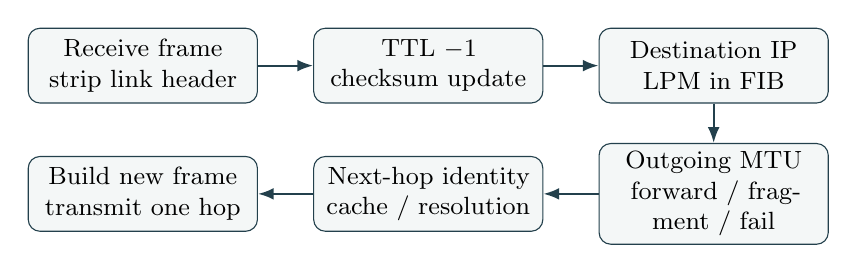
\begin{tikzpicture}[node distance=5mm and 7mm]
\node[net] (recv) {Receive frame\\strip link header};
\node[net,right=of recv] (life) {TTL $-1$\\checksum update};
\node[net,right=of life] (lookup) {Destination IP\\LPM in FIB};
\node[net,below=of lookup] (mtu) {Outgoing MTU\\forward / fragment / fail};
\node[net,left=of mtu] (neighbor) {Next-hop identity\\cache / resolution};
\node[net,left=of neighbor] (send) {Build new frame\\transmit one hop};
\draw[flow] (recv)--(life);
\draw[flow] (life)--(lookup);
\draw[flow] (lookup)--(mtu);
\draw[flow] (mtu)--(neighbor);
\draw[flow] (neighbor)--(send);
\end{tikzpicture}
\end{center}

这条生命周期有三个关键不变量：
\begin{enumerate}
  \item \kw{局部动作：}每台路由器只承诺把 packet 交给当前下一跳，不承诺自己持有完整端到端路径；
  \item \kw{作用域更新：}每跳重建 frame，TTL/Hop Limit 递减；无改写机制时端点 IP 语义保持；
  \item \kw{有限占用：}即使路由暂时形成 loop，TTL/Hop Limit 也让 packet 最终退出系统。
\end{enumerate}

TTL 不是实际秒数 deadline。IPv4 中 TTL 改变导致首部校验和更新；IPv6 使用 Hop Limit 且基础首部没有 header checksum。

\section{ARP、DHCP 与 ICMP：三种不同反馈}

\subsection{ARP：局部名字解析软状态}

ARP 缓存近似保存
\[
(IPv4\ next\!\!-hop\ address)\to(MAC\ address, age).
\]
缓存未命中时才需要在当前广播域请求。因缓存、链路类型和实现不同，“经过 $N$ 个路由器必然发生 $N+1$ 次 ARP”不是稳定规律。IPv6 使用 Neighbor Discovery，不应把 ARP 机制原样搬过去。

\subsection{DHCP：在没有配置时取得进入 IP 世界的条件}

\[
\text{DISCOVER}\to\text{OFFER}\to\text{REQUEST}\to\text{ACK}
\to\text{Bound}\to\text{Renew/Rebind/Expire}.
\]
DHCP 的输出不只是一个 IP，而是带期限的地址、prefix、gateway、DNS 等配置。广播和 UDP 服务于 bootstrap；它不是路由协议，也不负责之后每个 packet 的逐跳转发。

\subsection{ICMP：报告部分失败，不制造可靠性}

ICMP 可表达 Time Exceeded、Destination Unreachable、Echo、Packet Too Big 等反馈。它让端点观察到部分网络层事件，却不承诺每次错误都有通知：ICMP 本身可能丢失，且协议为避免反馈风暴而限制某些差错报文的生成。

\section{MTU 与 Fragmentation：尺寸冲突由谁承担}

\subsection{IPv4 教材模型}

若原始 IPv4 packet 超过输出链路 MTU，且 DF 等条件允许，source 或中间 router 可分片，最终 destination 才重组。若首部长度为 $H$，非最后片 payload 应取不超过 $MTU-H$ 的最大 8-byte 整数倍：
\[
Payload_{regular}=8\left\lfloor\frac{MTU-H}{8}\right\rfloor,
\qquad
Offset_i=\frac{\text{该片 payload 在原 payload 中的起始字节}}{8}.
\]
每片有自己的 total length；Identification 相同；除最后一片外 MF 为 1。任何一片丢失都会阻止整个原 packet 完成重组，这是分片放大成本。

\subsection{IPv6 改变责任 Owner}

IPv6 router 不在路径中分片。包过大时发送 ICMPv6 Packet Too Big；source 调整 packet size，必要时由 source 使用 Fragment extension header。准确表述是“router 不分片”，不是“IPv6 不允许分片”。

\begin{warnbox}{分片题的状态表}
逐片写 `payload bytes / total length / offset / MF`，总 payload 必须守恒；除最后片外检查 8-byte 对齐；再明确重组 Owner。只写一个分片公式而不推进每片状态，最容易在最后一片和 offset 上出错。
\end{warnbox}

\section{NAT：转发路径上的有状态改写}

NAPT 维护双向映射：
\[
(private\ IP,private\ port,protocol)
\leftrightarrow
(public\ IP,public\ port,protocol).
\]
出站 packet 触发或复用映射并改写 source tuple；返回 packet 必须用 public tuple 命中同一状态，恢复内部 endpoint。首部变化还会影响相关 checksum。

NAT 用地址复用换取 per-flow state、超时、入站建立困难和端到端透明性下降。它可能对未经邀请的入站流量形成阻碍，但 NAT 本身不等于完整 firewall policy，更不是 routing protocol。

\section{IPv6：地址空间、作用域与首部责任一起改变}

IPv6 具有 128-bit 地址、固定 40-byte 基础首部、extension header 链、Hop Limit 与 Next Header。它移除 IPv4 header checksum，把路径分片责任推回 source，并用 Neighbor Discovery 承担邻居发现。双栈与隧道是过渡策略类别，具体部署还可能有其他翻译组合；考试必须服从题设，不把某一种方案写成唯一现实。

\subsection{文本压缩必须可逆}

IPv6 地址由 8 组 16-bit 十六进制数组成。每组可删去前导零；一段连续全零组可用 \code{::} 压缩，但一个地址中只能出现一次，否则无法唯一恢复省略了多少组。做题时采用固定的反向检查：先数显式组数，再令 \code{::} 补足到 8 组，每组补齐 4 个十六进制位，最终应恰为 128 bit。

前缀仍写作 \code{address/prefix-length}。地址中出现全零组不改变前缀长度；“冒号位置”也不是网络号与接口号的天然边界，边界只由 prefix length 给出。

\subsection{地址类型先问“交付给几个接口”}

\begin{center}\small
\begin{tabularx}{\linewidth}{L{2.1cm}L{2.7cm}Y Y}
\toprule
类型 & 典型表示 & 交付语义 & 作用域/边界\\
\midrule
Unicast & global、\code{FE80::/10} 等 & 交给一个接口 & link-local 只在本链路使用，router 不跨链路转发\\
Anycast & 取自 unicast 空间 & 交给路由度量下的一个“最近”接口 & 语法上不能仅凭地址与 unicast 区分\\
Multicast & \code{FF00::/8} & 交给组内多个接口 & flags/scope/group ID 共同决定组语义\\
Special & \code{::/128}、\code{::1/128} & 未指定、回环 & 不能当普通可转发全局地址\\
\bottomrule
\end{tabularx}
\end{center}

IPv6 地址属于接口，不是“每台主机只能有一个地址”；同一接口可以同时拥有 link-local、global unicast 和若干 multicast 地址。IPv6 没有 broadcast，原来依赖广播的部分本地控制任务改用有明确作用域的 multicast，但这不等于“multicast 就是 broadcast 的改名”。

\section{IP Multicast：成员关系与分发路径是两个 Owner}

单播为每个接收者发送一份，广播向作用域内所有节点复制；组播把目标表示为 group，使网络只在通向成员的分叉处复制：
\[
\boxed{
\text{Sender sends once to Group G}
\to\text{Multicast distribution tree}
\to\text{replicate only at branches}
}.
\]
发送者不必是组成员；成员可动态加入或离开；组播仍继承 IP 的尽力而为语义，不因“一对多”自动具备可靠性或有序性。

IPv4 组播地址范围是 \code{224.0.0.0/4}，即最高四位为 \code{1110}；它标识接收者组，不是某台单一主机。IPv6 multicast 使用 \code{FF00::/8}，其中 scope 字段限制组的作用范围。地址范围只回答“目标属于哪个组/作用域”，不能单独生成从 source 到所有成员网络的分发路径。

完整组播系统至少含两个不同问题：
\begin{enumerate}
  \item \kw{Local membership：}主机与本地 multicast router 之间维护“本链路是否还有 group $G$ 的接收者”。IPv4 教材模型由 IGMP 承担；query/report/leave 改变的是成员软状态。
  \item \kw{Inter-router delivery：}路由器之间构造到各成员网络的无环分发状态，使分组只沿需要的接口复制。具体组播路由协议不由 IGMP 代替。
\end{enumerate}

组播转发不能直接照搬普通单播的“只按 destination 做一次 LPM”。其核心检查通常是：分组是否从到达 source 的合理反向接口进入，以及应复制到哪些有下游成员的 outgoing interfaces。408 若只考基本概念，应写清 \textbf{membership state $\neq$ distribution-tree state}，不擅自展开考纲外协议细节。

\section{408 常见网络层协议流程：按报文推进}

前面的章节给出了机制边界；本节补上题目中常要求逐步填写的报文流程。每条流程都先写触发条件，再写报文携带的关键字段，最后写状态由谁改变。

\subsection{IPv4/IPv6 首部：字段怎样服务转发}

\begin{center}\small
\begin{tabularx}{\linewidth}{L{2.3cm}Y Y}
\toprule
首部对象 & 408 常考字段 & 字段在流程中的作用\\
\midrule
IPv4 基础首部 & Version、IHL、Total Length、Identification、Flags、Fragment Offset、TTL、Protocol、Header Checksum、Source/Destination & 路由器检查长度与 TTL；分片使用三元组；Protocol 交给上层；TTL 变化后 checksum 必须重算\\
IPv6 基础首部 & Version、Traffic Class、Flow Label、Payload Length、Next Header、Hop Limit、Source/Destination & 固定基础首部便于转发；Next Header 串接扩展/上层；路径 router 不分片且无 header checksum\\
\bottomrule
\end{tabularx}\end{center}

不要把 IP 首部字段默写成“每跳都变”：通常变化的是 TTL/Hop Limit、IPv4 checksum，以及分片或 NAT 等机制明确改写的字段；Source/Destination IP 在无 NAT、隧道或移动性扩展时保持端点语义。

\subsection{ARP：同网段与异网段的请求--应答}

\[
\begin{array}{l}
\text{Host decides next-hop IP}\\
\to\text{ARP Request: broadcast, target protocol address = next-hop IP}\\
\to\text{owner sends ARP Reply: unicast, sender IP/MAC binding}\\
\to\text{cache binding with aging}\\
\to\text{encapsulate packet in frame and send.}
\end{array}
\]
同网段时 next-hop IP 是最终 destination IP；异网段时是 default gateway。Request 在当前广播域内传播，router 不转发 ARP 广播。题目若给“缓存已命中”，应跳过 Request；若题目换成 IPv6，协议对象转为 Neighbor Discovery。

\subsection{DHCP：DORA 与租约生命周期}

新 client 尚无可用地址时，经典流程为：
\[
\begin{gathered}
\text{DHCPDISCOVER (broadcast)}\to\text{DHCPOFFER}\to\text{DHCPREQUEST (选择 server)}\\
\to\text{DHCPACK (lease/config)}.
\end{gathered}
\]
DISCOVER 找服务；OFFER 提供 proposed IP、lease 与配置；REQUEST 明确选择哪个 offer；ACK 使 client 进入 Bound。租约未到期前发送 renew REQUEST；续租失败再进入 Rebind；最终过期则释放配置并重新发现。DHCP 的 server identifier、requested IP、lease time、subnet mask、router、DNS 等选项是配置证据，不是普通 IP forwarding 表项。

\subsection{ICMP：错误与诊断反馈}

\begin{center}\small
\begin{tabularx}{\linewidth}{L{3.2cm}Y Y}
\toprule
触发 & 典型 ICMP 报文 & 接收方如何使用\\
\midrule
TTL/Hop Limit 耗尽 & Time Exceeded & traceroute 观察该跳；源端不因此获得可靠传输承诺\\
无路由/端口/策略拒绝 & Destination Unreachable & 区分网络、主机、协议/端口或分片相关原因（服从题设）\\
Echo 诊断 & Echo Request/Reply & ping 检查可达性与往返时间，不等同应用服务可用\\
IPv6 packet 超过路径 MTU & Packet Too Big & source 更新 PMTU/packet size；router 不分片\\
\bottomrule
\end{tabularx}\end{center}
ICMP 是反馈路径，不是 ACK；它可能丢失，也不能替代 TCP/ARQ 的重传状态。

\subsection{IPv4 分片：一个数值流程}

设原 payload 为 $4000$ B，IPv4 首部 $H=20$ B，输出 MTU 为 $1500$ B，允许分片。每个非末片最多承载 $1480$ B，于是：
\[
\begin{array}{c|c|c|c|c}
片 & payload & total\ length & offset & MF\\\hline
1&1480&1500&0&1\\
2&1480&1500&185&1\\
3&1040&1060&370&0
\end{array}
\]
三个 fragment 共享 Identification；offset 以 8 B 为单位；最终 destination 依据 Identification、Source/Destination 和 Protocol 等信息重组。任一片丢失都会使原始 datagram 交付失败。若题设 DF=1 或 IPv6 router 分片，流程转为 ICMP/PMTU 分支。

\subsection{NAT/NAPT：出站建表与返回匹配}

\[
\begin{gathered}
\text{private tuple arrives}\to\text{allocate public tuple}\to\text{rewrite source}\to\text{forward}\\
\text{return packet hits public tuple}\to\text{lookup mapping}\to\text{rewrite destination}\to\text{deliver internal endpoint}.
\end{gathered}
\]
题目应同时维护映射表、空闲/超时状态和 checksum 影响。没有 public tuple 命中时，入站 packet 通常不能仅凭目的 public IP 推出内部 endpoint；这解释了 NAT 的入站可达性边界。

\subsection{IPv6 Neighbor Discovery：ARP 的替代接口}

在 408 题设中可将其抽象为：节点用 Neighbor Solicitation 查询邻居链路地址，邻居用 Neighbor Advertisement 响应；Router Solicitation/Advertisement 还可帮助主机获得前缀、默认路由等配置。它们仍然服务“当前一跳身份/配置”，不能因此把 IPv6 邻居发现写成跨网路由协议。

\section{Mobile IP：用绑定把稳定身份接到当前位置}

固定 IP 同时被当成“谁”和“在哪里”时，节点换网会产生冲突：保持地址会破坏拓扑聚合，改地址又会破坏持续身份。Mobile IP 的最小母模型是：
\[
\boxed{\text{Stable home identity}\ne\text{Current care-of locator}}
\]
移动节点向锚点/归属机制登记 binding；发往稳定身份的流量可被截获并隧道到当前 locator，形成潜在 triangle routing、额外状态和故障依赖。

经典 Mobile IPv4 把这条抽象落实为四个角色：mobile node（MN）、home agent（HA）、可选 foreign agent（FA）与 correspondent node（CN）。home address 维持持续身份，care-of address（CoA）表示当前隧道终点；CoA 可以是 FA 提供的 foreign-agent CoA，也可以是 MN 自己取得的 co-located CoA。

\begin{enumerate}
  \item \kw{Agent discovery：}HA/FA 发送 Agent Advertisement，MN 也可 Solicitation；MN 据此判断自己在 home network 还是 foreign network，并取得可用 CoA。
  \item \kw{Registration：}离家后，MN 直接或经 FA 向 HA 发 Registration Request；HA 验证后建立带 lifetime 的 $home\ address\to CoA$ binding，并返回 Registration Reply。失败或超时不能进入可用绑定状态。
  \item \kw{Tunneling：}CN 仍把数据报发往 home address；HA 在 home network 截获，将原 datagram 封装进外层 datagram，外层 destination 为 CoA；隧道终点解封装后交给 MN。
  \item \kw{Return/deregister：}MN 回到 home network 后注销旧绑定，恢复普通路由交付，避免继续绕经旧 CoA。
\end{enumerate}

基本模型的正向路径可能是 $CN\to HA\to CoA\to MN$，反向却由 MN 按普通路由直接发往 CN，形成 triangle routing。它不是路由环，而是稳定身份经锚点重定向造成的路径不对称。隧道的外层地址服务 locator，内层 home address 保留端点语义；解题必须分别推进两层 TTL、长度/MTU 与封装状态。

这里保留的是“身份--位置分离、绑定、锚点、隧道”的可复用结构。经典 Mobile IP 的 Home Agent/Foreign Agent 与蜂窝核心网中的 HSS、P-GW 等组件不具有稳定的一一等价关系，不能因为功能相似就直接换名。

\section{五列概念边界}

\begin{center}
\small
\begin{tabularx}{\linewidth}{L{1.75cm}C{0.35cm}L{1.75cm}Y Y}
\toprule
概念 A & $\neq$ & 概念 B & 真正区别与题面信号 & 混淆后果\\
\midrule
Destination IP & $\neq$ & Next-hop IP & 最终三层目标 vs 当前节点的交付对象；先做 same-subnet/LPM & 跨网段 ARP 错对象\\
Next-hop IP & $\neq$ & MAC & 三层转发动作 vs 当前链路身份 & 把 route table 写成 MAC table\\
RIB selection & $\neq$ & FIB lookup & 控制面选路/安装 vs packet 到达时 LPM & 把 metric 与 LPM 混算\\
Subnet & $\neq$ & VLAN & 三层 prefix 作用域 vs 二层广播作用域 & 误认为天然一一对应\\
TTL & $\neq$ & Deadline & 逐跳生命预算 vs 真实时间限制 & 用秒解释 TTL\\
Fragmentation & $\neq$ & Segmentation & IP 适配 MTU vs transport 构造传输单元 & 字段和重组 Owner 错\\
NAT & $\neq$ & Routing & tuple 改写和映射 vs 下一跳选择 & 漏掉反向状态\\
Home identity & $\neq$ & Locator & 持续身份 vs 当前拓扑位置 & 移动时把换网等同换身份\\
IGMP membership & $\neq$ & Multicast routing & 本地链路组成员状态 vs 路由器间分发状态 & 用一次 Join 直接生成全网树\\
Routing processor & $\neq$ & Switching fabric & 生成/安装控制状态 vs 搬运已查表分组 & 认为每包都运行 OSPF/BGP\\
\bottomrule
\end{tabularx}
\end{center}

\section{Correctness、Cost 与 Tradeoff}

\begin{center}
\small
\begin{tabularx}{\linewidth}{L{2.4cm}Y Y Y}
\toprule
机制 & 获得的能力 & 主要状态/成本 & 边界\\
\midrule
CIDR/aggregation & 压缩地址与转发状态 & 分配对齐、摘要可能隐藏细节 & 更具体前缀仍可例外\\
LPM & 对重叠前缀选最具体动作 & 快速查找结构 & 依赖已安装 FIB\\
ARP/DHCP & 本地身份解析与启动配置 & cache/lease、广播、老化 & 受链路/广播域限制\\
TTL/ICMP & 限制循环并提供反馈 & 丢弃、反馈流量 & 不保证通知到达\\
Fragmentation & 适配异构 MTU & 首部、重组、丢片放大 & IPv4/IPv6 Owner 不同\\
NAT & 复用 IPv4 地址 & per-flow mapping、超时、改写 & 降低端到端透明性\\
Mobile anchor & 身份与位置解耦 & binding、tunnel、绕路 & 仅作扩展关系\\
Multicast & 在分叉点复制到动态成员组 & membership 与 tree state & 不保证可靠/有序，也不等于广播\\
Router queues & 吸收瞬时到达与速率不匹配 & 排队时延、HOL、有限 buffer & 持续超载最终丢包\\
\bottomrule
\end{tabularx}
\end{center}

\section{做题控制协议与 First Divergence}

\begin{enumerate}
  \item 写当前节点：host、router、DHCP client/server 还是 NAT middlebox；
  \item 写当前作用域和名字类型：destination IP、next-hop IP、MAC 或 tuple；
  \item host 先做 same-subnet，router 对已安装 FIB 做 LPM；
  \item 明确 next-hop IP 后，才判断邻居缓存是否命中、是否需要解析；
  \item 逐跳维护 TTL/Hop Limit、frame 地址以及必要的 checksum；
  \item 比较 packet size 与 outgoing MTU，声明 IPv4/IPv6 和 DF/PMTU 条件；
  \item NAT 维护正反向 tuple；分片维护逐片状态表；
  \item IPv6 地址先恢复 8 组并判作用域；组播分开 membership 与 distribution state；
  \item Mobile IP 分开内外层地址，并逐步检查 discovery、registration、tunnel 与 deregistration；
  \item 路由器组成题逐包追踪 input queue、FIB lookup、fabric、output queue 与 link transmit；
  \item 用“哪个 Owner 在什么事件后更新了什么状态”复核答案。
\end{enumerate}

\begin{warnbox}{高频 First Divergence}
先 ARP 最终目的 IP，说明漏了 same-subnet 分叉；LPM 后又拿不同长度前缀的 metric 混排，说明混淆了具体性与选路；认为每跳都改变目的 IP，说明把 frame 重封装投射到 packet；写“IPv6 不能分片”，说明没有区分 router 与 source；一个地址写两个 \code{::}，说明丢失可逆性；把 IGMP 当成组播路由算法，说明混淆本地成员与全网分发；把 HA 与 FA 当成必经同一设备，说明没有识别两类 CoA；写“NAT 就是防火墙”，说明没有识别映射状态与安全策略的边界。
\end{warnbox}

\section{考纲映射、来源处理与一页复原}

\begin{center}
\small
\begin{tabularx}{\linewidth}{L{3.2cm}Y Y}
\toprule
旧笔记主题 & 本册归宿 & 处理结论\\
\midrule
IPv4、CIDR、子网与路由基础 & prefix/same-subnet/LPM & Canonical，补足 RIB/FIB 边界\\
ARP、DHCP、ICMP、NAT & 局部解析、启动、反馈、改写 & Canonical，删除固定 ARP 次数等绝对化\\
IPv4/IPv6 分片 & MTU 责任模型 & Canonical，修正“IPv6 不允许分片”\\
Mobile IP & 身份--位置分离、发现/注册/隧道 & Canonical 408 Core，拒绝蜂窝组件硬等同\\
IPv6 地址、IP multicast、router composition & 地址作用域、成员/分发、数据平面 & Canonical，本轮考纲审计补齐\\
设备表、交换表、路由协议 & NET-02/NET-05 & 只建立接口，不重复拥有\\
\bottomrule
\end{tabularx}
\end{center}

\begin{corebox}{一页压缩}
\[
\boxed{\begin{gathered}
\text{先定 Scope}\to\text{识别名字类型}\to\text{用 Prefix 得到 Next Hop}\\
\to\text{解析当前链路身份}\to\text{推进 packet/frame 状态}
\end{gathered}}
\]
复原本册时回答：为什么 prefix 能压缩状态？Same-subnet 怎样决定 ARP 对象？RIB 与 FIB 分别是谁的输出？输入/交换结构/输出分别承担什么？IPv6 地址怎样从文本恢复并判作用域？IPv4/IPv6 的分片 Owner 有何不同？组播成员与分发状态由谁维护？Mobile IP 怎样用 binding 与 tunnel 连接 home identity 和 CoA？
\end{corebox}

\end{document}
